\title{
Higgs exotic decays into long-lived particles
}



%========================================
\subsubsection{Higgs exotic decays into long-lived particles}\label{Sec:9.1.2}
\begin{center}{\it by Jia Liu, Zhen Liu, Lian-Tao Wang}
\end{center}


The Higgs boson is a well-motivated portal to new physics sectors, introducing a vast variety of exotic decays~\cite{Curtin:2013fra}.
The presence of long-lived particles (LLP) can be a striking feature of many new physics models~\cite{Liu:2018wte,Barbier:2004ez,Giudice:1998bp,Meade:2010ji,Arvanitaki:2012ps,ArkaniHamed:2012gw,Liu:2015bma,Chacko:2005pe, Burdman:2006tz,Kang:2008ea,Craig:2015pha, Davoli:2017swj}. 
At the same time, vast swaths of the possible parameter space of the LLP remain unexplored by LHC searches.
LHC general purpose detectors, ATLAS and CMS, provide full angular coverage and sizable volume, making them ideal for LLP searches.
However, searches for LLPs that decay within a few centimeter of the interaction point suffer from large SM backgrounds. 
LLPs produced at the LHC generically travel slower than the SM background and decay at macroscopic distances away from the interaction point. Hence, they arrive at outer particle detectors with a sizable time delay. 

Recently, precision timing upgrades with a timing resolution of 30 picoseconds have been proposed to reduce pile-up for the upcoming 
runs with higher luminosity, including MIP Timing Detector (MTD)~\cite{Collaboration:2296612}  by the CMS collaboration for 
the barrel and endcap region in front of the electromagnetic calorimeter, the High Granularity Timing Detector~\cite{Allaire:2018bof} 
by the ATLAS collaboration in endcap and forward region,  and similarly multiple precision timing upgrades~\cite{Bediaga:2018lhg} by the 
LHCb collaboration.
As a strategy applicable to a broad range of models, we propose the use of a generic Initial State Radiation (ISR) jet to timestamp the hard collision and require only a single LLP decay inside the detector with significant time delay. Such a strategy can greatly suppress the SM background and 
reach a sensitivity two orders of magnitude or more better than traditional searches in a very larger parameter space~\cite{Aad:2015uaa, CMS:2014wda,Coccaro:2016lnz, Liu:2015bma}. 
With a general triggering and search strategy that can capture most LLP decays, 
we show a striking improvement in sensitivity and coverage for LLPs. In addition to the MTD at CMS, we also consider a hypothetical timing layer on the outside of the ATLAS Muon Spectrometer (MS) as an estimate of the best achievable reach of our proposal for LLPs with long lifetimes.  \\

Higgs decaying to glueballs with subsequent decays into SM jet pairs is our benchmark model here. This occurs in model~\cite{Craig:2015pha} where the Higgs is the portal to a dark QCD sector whose lightest states are the long-lived glueballs. 
Typical energy of the glueball is set by the Higgs mass, and the time delay depends on glueball mass. 
Timestamping the hard collision is achieved by using an ISR jet: 
\bea
pp\rightarrow h+j&,\ h\rightarrow X+X,\ X\rightarrow {\rm SM},   %,\\
%\rm{SigB:}& \ pp\rightarrow \tilde \chi \tilde \chi+j&,\ \tilde \chi^0_1 \to h+\tilde G \to {\rm SM}+\tilde G.
\eea
where $X$ represents the LLP.

While particle identification and kinematic reconstruction are highly developed,  
usage of timing information has so far been limited since prompt signatures are often assumed. 
Such an assumption could miss a crucial potential signature of an LLP, a significant time delay. 
Here we outline a general BSM signal search strategy that uses the timing information
and the corresponding background consideration.
A typical signal event of LLP is shown in the left panel of Fig.~\ref{fig:ctaulimitHiggs}. 
The LLP, $X$, travels a distance $\ell_X$ into a detector volume and decays into two light SM particles 
$a$ and $b$, which then reach timing detector at a transverse distance $L_{T_2}$ away from the beam axis. Typically, the SM particles travel at velocities close to the speed of light.
For simplicity, we consider neutral LLP signals where background from charged particles can be vetoed using 
particle identification and isolation.
The decay products of $X$ arrive at the timing layer with a time delay
$
\Delta t^i_{\rm delay} = \frac{\ell_X}{\beta_X} + \frac{\ell_i}{\beta_i} - \frac{\ell_{\rm SM}}{\beta_{\rm SM}}
%\label{eq:delaysimple}
$
for $i$th decay products from $X$ and $\beta_i \simeq \beta_{\rm SM} \simeq 1 $. 
It is necessary to have prompt particles from production or decay, or ISR, which arrives at timing layer with 
the speed of light, to derive the time of the hard collision at the primary vertex (to ``timestamp'' the hard collision).\\


\begin{figure}[t]
    \centering
    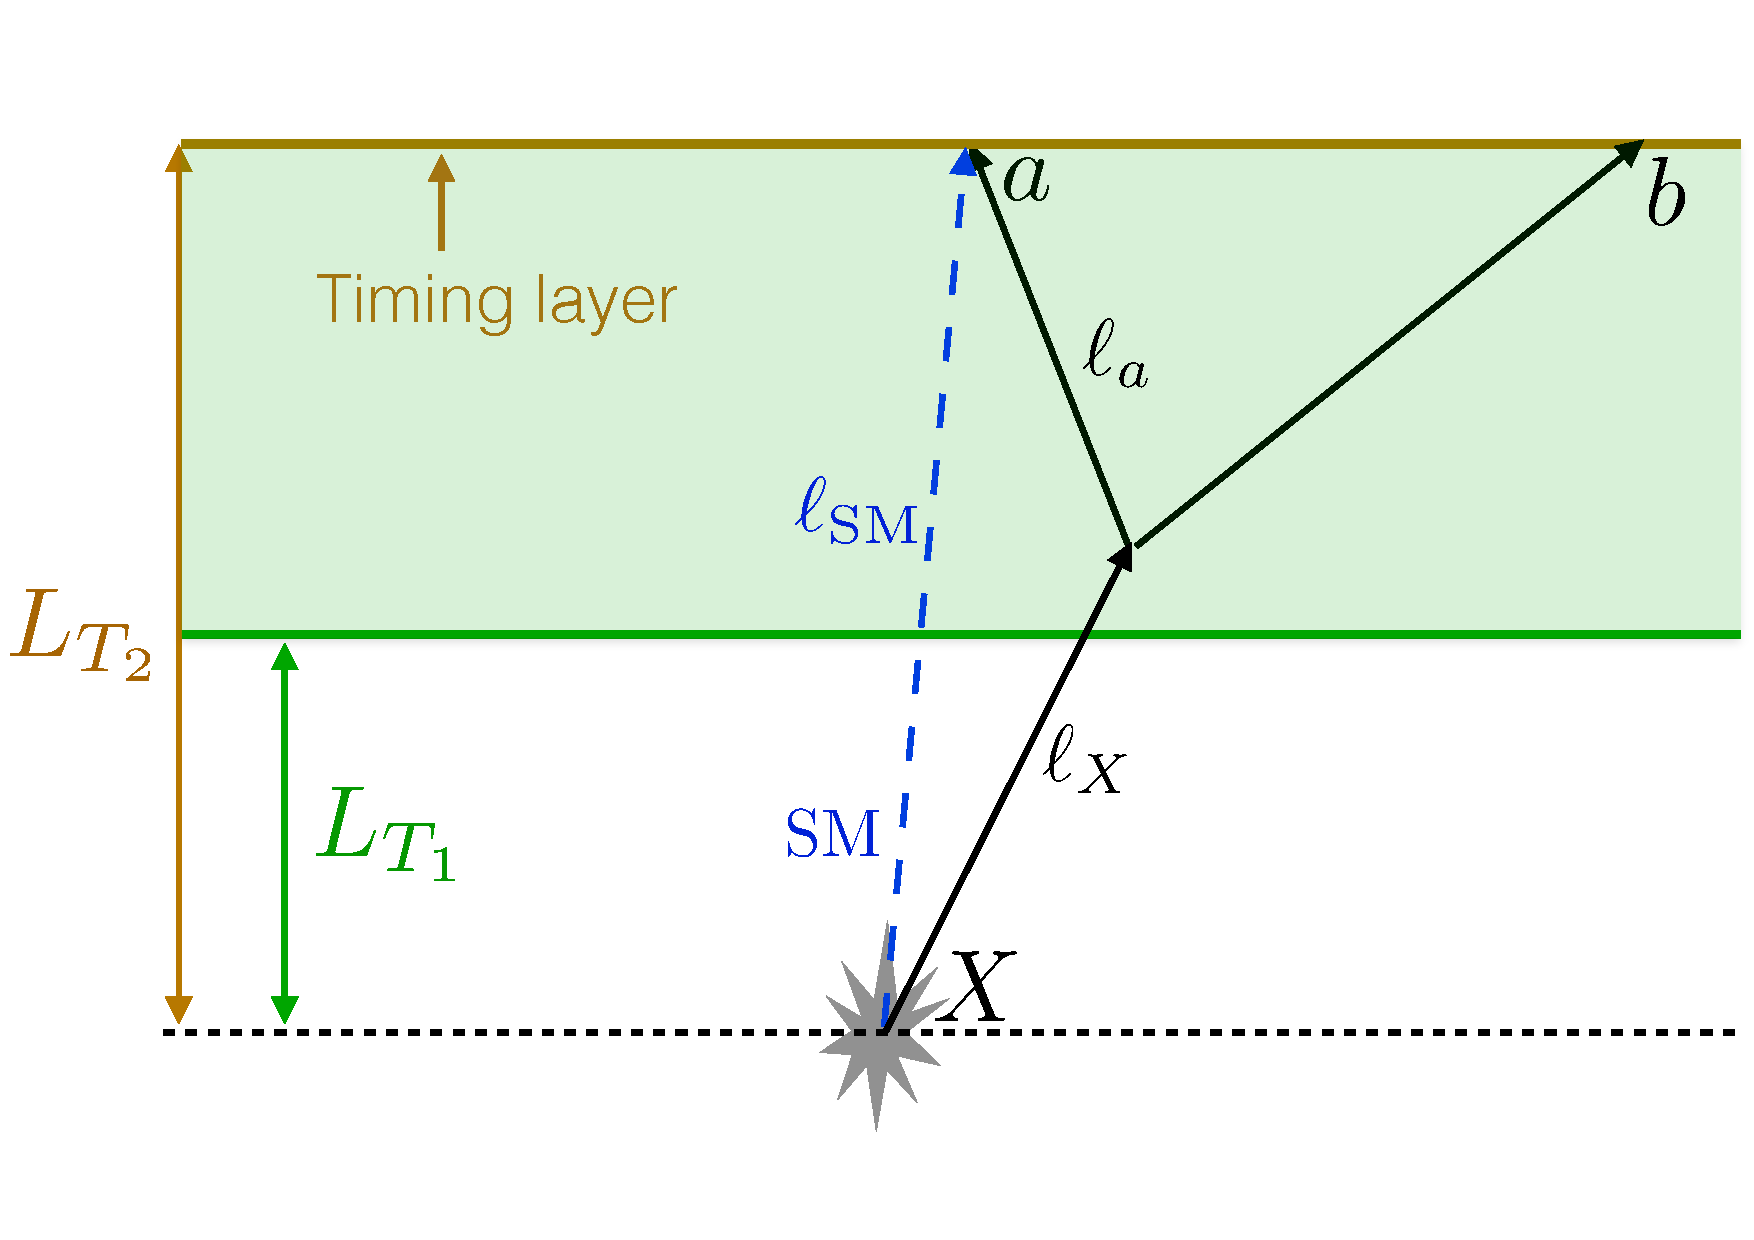
\includegraphics[width=0.45\columnwidth]{\main/section9/plots/schematic_drawing} 
    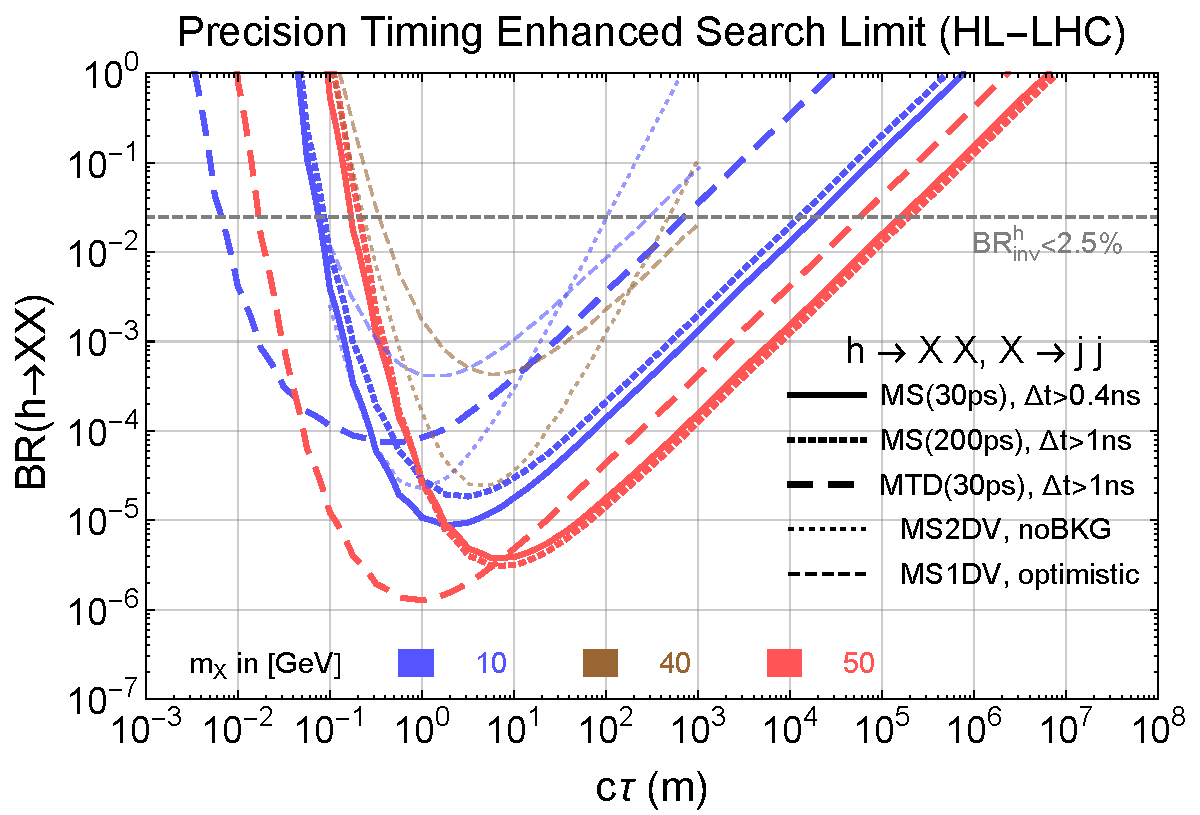
\includegraphics[width=0.45\columnwidth]{\main/section9/plots/10-20-50-MC-Lcalc-BRlimit-with-deltaT-cut-MS-1ns-eEta5-beta-added} 
    \caption{ Left Panel: An event topology with an LLP $X$ decaying into two light SM particles $a$ and $b$. A timing 
    layer, at a transverse distance $L_{T_2}$ away from the beam axis (horizontal gray dotted line), is placed at the end of the detector volume 
    (shaded region). The trajectory of a reference SM background particle is also shown (blue dashed line).
    The gray polygon indicates the primary vertex.
    Right Panel: the $95\%$ C.L. limit on $\text{BR}(h \to XX)$ for signal process $pp \to j h$ with subsequent decay 
    $h\to X X$ and $X \to j j$. Different colors indicate different masses of the particle $X$. 
    The thick solid and dotted (thick long-dashed) lines indicate MS (MTD) searches with different timing cuts. The numbers in parentheses are 
    the assumed timing resolutions. Other 13 TeV LHC projections \cite{Coccaro:2016lnz, Bernaciak:2014pna} are plotted in thin lines. Figures are taken from Ref.~\cite{Liu:2018wte}.
    }
    \label{fig:ctaulimitHiggs}
\end{figure}

We consider events with at least one ISR jet to timestamp the primary vertex (PV) and one delayed SM object coming from the LLP decay. We propose two searches using the time delay information:
\begin{center}
	\scalebox{0.95}{
    \begin{tabular}{|c|c|c|c|c|c|c|c|}
        \hline
        & $L_{T_2}$ & $L_{T_1}$ & Trigger & $\epsilon_{\rm trig}$ & $\epsilon_{\rm sig}$ & $\epsilon_{\rm fake}^{j}$ & Ref. \\ \hline
        MTD & 1.17 m & 0.2 m & DelayJet & 0.5 & 0.5 & $10^{-3}$ & \cite{Collaboration:2296612} 
        \\ \hline
        MS & 10.6 m & 4.2 m & MS RoI & 0.25, 0.5 & 0.25 & $5.2\times 10^{-9}$ & \cite{Aad:2015uaa}
        \\
        \hline
    \end{tabular}}
\end{center}
The size of the detector volume is described by transverse distance to the beam pipe from $L_{T_1}$ to $L_{T_2}$, where the timing layer
is located. For both searches, we assume a similar timing resolution of 30~ps.
For the MS search, because of the larger time delay and much less background due to ``shielding'' by inner detectors, 
a time resolution of 0.2 - 2 ns could achieve a similar physics reach. The $\epsilon_{\rm trig}$, 
$\epsilon_{\rm sig}$ and $\epsilon_{\rm fake}^j$ are the efficiencies for trigger, signal selection and a QCD jet faking the delayed jet signal with $p_T>30$~GeV in MTD and MS searches, respectively. 

For the MTD search, we assume a new trigger strategy of a delayed jet using the CMS MTD.
This can be realized by putting a minimal time delay cut when comparing the prompt timestamping jet with $p_T > 30$~GeV with the arrival time of another jet at the timing layer. 
The MTD signal, after requiring minimal decay transverse distance of 0.2 m ($L_{T_1}$), will not 
have good tracks associated with it. Hence, the major SM background is from trackless jets.
The jet fake rate of $\epsilon_{\rm fake}^{\rm j, MTD} = 10^{-3}$ is estimated
using {\tt Pythia}~\cite{Sjostrand:2007gs} by simulating the jets with minimal $p_T$ of 30~GeV and studying the anti-kt jets with $R=0.4$, where all charged constituent hadrons are too soft ($p_T<1~\GeV$). 
For the MS search, we use the MS Region 
of Interest (MS RoI) trigger from a very similar search~\cite{Aaboud:2017iio} as a reference, with an efficiency 
of $\epsilon_{\rm trig}=0.25$ and 0.5 for the two benchmark BSM signals, and a signal selection efficiency of 
$\epsilon_{\rm sig}=0.25$. The backgrounds are mainly from the punch-through jets, and the  fake efficiency can be inferred 
to be $\epsilon_{\rm fake}^{\rm j, MS} = 5.2 \times 10^{-9}$, normalized to 1300 fake MS barrel events at 8 TeV~\cite{Aaboud:2017iio}.
For detailed discussion on the background estimation, see Ref.~\cite{Liu:2018wte}.
\\

To emphasize the power of timing, we rely mostly on the timing information to suppress background and make only 
minimal cuts. We only require one low $p_T$ ISR jet, with $p_T^j > 30~\text{GeV}$ and $|\eta_j| < 2.5$.
In both signal benchmarks, we require that at least one LLP decays inside the detector. We generate signal events using {\tt MadGraph5}~\cite{Alwall:2014hca} at parton level. 
After detailed simulations of the delayed arrival time, we derive the projected sensitivity using the 
cross-sections obtained in Ref.~\cite{Greiner:2015jha}. The $95\%$ C.L. sensitivity is shown in Fig.~\ref{fig:ctaulimitHiggs}. 
We assume $X$ decays to SM jet pairs with 100\% branching fraction.
The MTD and MS searches, with $30$ ps timing resolution, are plotted in thick dashed and solid lines, respectively. 
For MS, the best reach of $\text{BR}(h\to XX)$ is about a few times $10^{-6}$ for $c \tau \sim 10$~m. 
The reach is relatively insensitive to the mass of $X$ when $m_X> 10$~GeV because $X$ are moving slowly enough
to pass the timing cut. 
For the MS search, a less precise timing resolution 
($200$ ps) has also been considered with cut $\Delta t > 1$ ns. After the cut, the backgrounds from same-vertex hard collision (SV) and pile-up (PU) for MS search are $0.11$ and $7.0 \times 10^{-3}$ respectively, and the SV background dominates.  
The reach for heavy $X$ is almost not affected, 
while reduced by a factor of around two for light X.

In the right panel of Fig.~\ref{fig:ctaulimitHiggs}, we compare MTD and MS (thick lines) with 13 TeV  HL-LHC (with $3 ~\text{ab}^{-1}$ integrated luminosity) projections, two displaced vertex (DV) at 
MS using zero background assumption (thin dotted) and one DV at MS using a data-driven method with optimistic background estimation (thin dashed) from \cite{Coccaro:2016lnz}. 
The projected limits from invisible Higgs decay at the 14 TeV HL-LHC (see Sec. \ref{sec6:exp} of this report) is also shown in the right panel of Fig.~\ref{fig:ctaulimitHiggs}. \\

Exploiting timing information can significantly enhance 
the sensitivities of LLP searches at the HL-LHC. 
To emphasize the advantage of timing, we made minimal requirements on the signal, with one ISR jet
and a delayed signal. 
The temporal behavior of the SM and detector background are not yet well understood. This novel investigation~\cite{Liu:2018wte} requires further studies on the background behaviors at the HL- and HE-LHC to further realize the proposed trigger and analysis.
Further optimization can be developed for more dedicated searches. 
The timestamping ISR jet can be replaced by other objects, such as leptons or photons. Depending on the underlying signal 
and model parameters, one can also use prompt objects from signal production and decay. In addition, for specific searches, 
one could also optimize the selection of the signal based on the decay products of LLPs. 
Finally, we emphasize that the current LLP searches are complimentary to the timing based searches discussed here. Once combined,
the current searches should in general gain better sensitivity for heavy LLP. These future perspectives can be further extended and realized at the HE-LHC with more advanced phenomenological studies with detector, trigger and analysis, as well as higher statistics on the Higgs bosons.


